% DOC SETTINGS ===================================
\documentclass{article}
\usepackage[utf8]{inputenc}
\usepackage{steinmetz}
\usepackage{mathtools}  
\usepackage{multicol}
\usepackage{circuitikz}
\usepackage{tikz}
\usepackage{listings}
\usepackage{geometry}
\usepackage{fancyhdr}
\usepackage{amsfonts}
\usepackage{media9}
\usepackage{parskip}
\usetikzlibrary{positioning, fit, calc}
\pagestyle{fancy}
\lhead{VISA Address}
\rhead{Kavin Thirukonda 2021}
\PassOptionsToPackage{hyphens}{url}\usepackage{hyperref}
\hypersetup{
    colorlinks=true,
    linkcolor=blue,
    filecolor=magenta,      
    urlcolor=cyan,
}
\fancyheadoffset{0mm}
 \geometry{
 a4paper,
 total={170mm,257mm},
 left=20mm,
 top=25mm,
 }
\usepackage{listings}
\usepackage[]{color}
\definecolor{codegreen}{rgb}{0,0.6,0}
\definecolor{codegray}{rgb}{0.5,0.5,0.5}
\definecolor{codepurple}{rgb}{0.58,0,0.82}
\definecolor{backcolour}{rgb}{0.95,0.95,0.92}
\mathtoolsset{showonlyrefs} 
\cfoot{}
% DOC SETTINGS ===================================
\begin{document}
\section*{Preface}
\begin{center}
    Since the 82357B is not a NI product and is not native, it can be sometimes difficult to interface to LabView unlike VEE, so the procedure would be different every time depending on the computers installed programs. The NI equivalent of the 82357B is:
    
    \url{https://www.ni.com/en-us/support/model.gpib-usb-hs.html}
\end{center}
\section*{OS Requirements}
\subsection*{Windows}
\begin{itemize}
    \item Windows 10 (32\&64 Bit)
    \item Windows 8 and 8.1 (32\&64 Bit)
    \item Windows 7 SP1 (32\&64 Bit)
    \item Windows Server 2012 (64 Bit)
    \item Windows Server 2008 R1 SP1 (64 Bit)
\end{itemize}
\subsection*{Linux}
\begin{itemize}
    \item 64 Bit Red Hat Enterprise 7.1 - 7.5
    \item 64 Bit CentOS 7.1 - 7.5
\end{itemize}
\section*{Other Prerequisites}
\begin{itemize}
    \item The 82357B USB-to-GPIB inteface must be plugged in to the computer as well as the instrument.
    \item LabView must be fully installed
\end{itemize}
\newpage
\section*{Keysight IO Libraries Suite}
\begin{enumerate}
    \item Download IO Libraries Suite
    Download the latest version of IO Libraries Suite at:
    \begin{center}
        \url{http://www.keysight.com/find/iosuite}
    \end{center}
    Click preferred version to download, both standard and expert will work fine.
    
    \vspace{.1in}
    \begin{center}
        \boxed{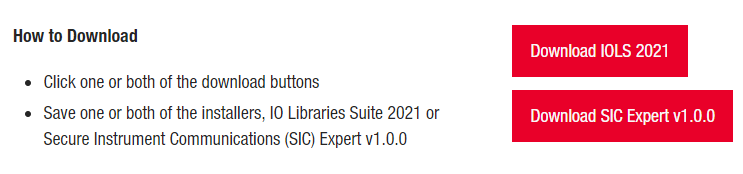
\includegraphics[width = .75\textwidth]{images/download.png}}
    \end{center}
    \vspace{.1in}
    \item Fill out the download form and click download.
    
    \vspace{.1in}
    \begin{center}
        \boxed{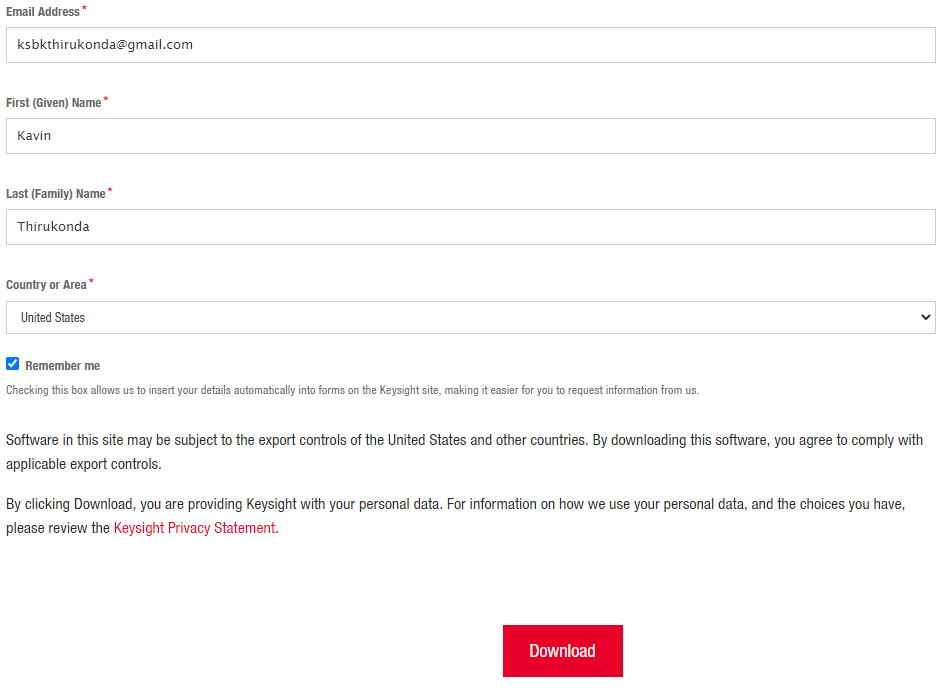
\includegraphics[width = .75\textwidth]{images/download-form.png}}
    \end{center}
    \vspace{.1in}
    
    \item Once the .exe has been opened, go through a standard install without changing any settings from default.
    
    \vspace{.1in}
    \begin{center}
        \boxed{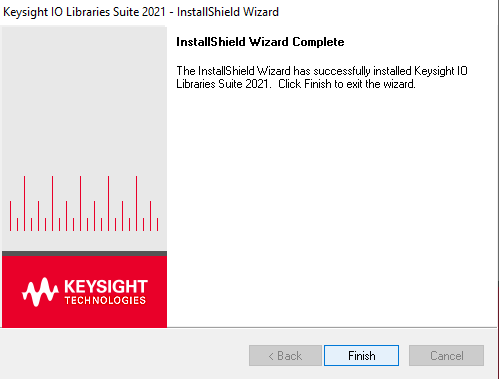
\includegraphics[width = .55\textwidth]{images/download-complete.png}}
    \end{center}
\end{enumerate}
    \newpage
    \section*{NI Max}
    \begin{enumerate}
        \item To allow for communication between the 82357B we need to enable tulip, to start we go to labview and navigate to measurement and automation explorer
        
        \vspace{.1in}
        \begin{center}
            \boxed{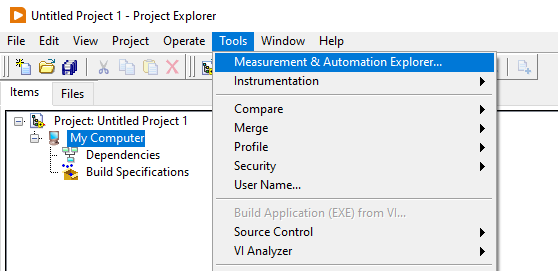
\includegraphics[width = .65\textwidth]{images/open.png}}
        \end{center}
        \vspace{.1in}

        \item Once the program opens, navigate to VISA options
        
        \vspace{.1in}
        \begin{center}
            \boxed{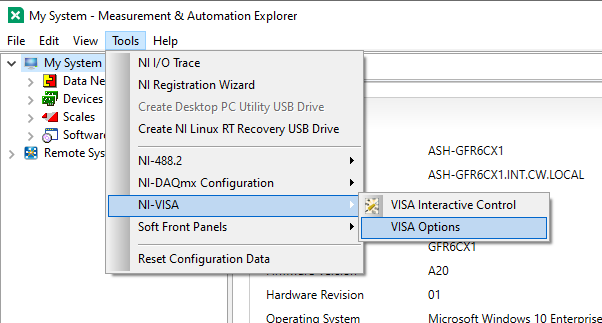
\includegraphics[width = .65\textwidth]{images/options.png}}
        \end{center}
        \vspace{.1in}
        
        \item Then under general settings, click passports and make sure tulip is enabled, such that the checkbox is marked.
        
        \vspace{.1in}
        \begin{center}
            \boxed{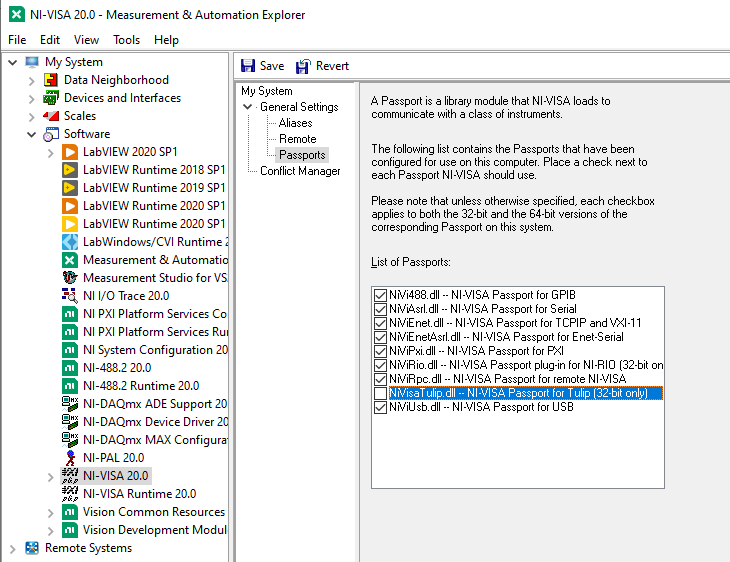
\includegraphics[width = .65\textwidth]{images/tulip.png}}
        \end{center}
        \vspace{.1in}
    \end{enumerate}
    \newpage
    
    \begin{center}
        Now the VISA address of all connected devices can be viewed and used under devices and interfaces by giving a labview module the valid VISA address.
    \end{center}
    \vspace{.1in}
        \begin{center}
            \boxed{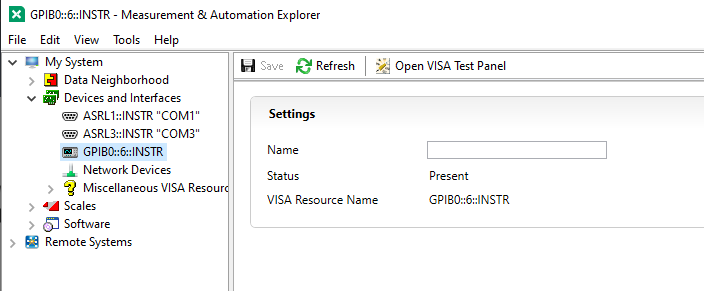
\includegraphics[width = .65\textwidth]{images/address.png}}
        \end{center}
        \vspace{.1in}
\end{document} 